\section{Communication protocols}
\label{sec:comm_protocols}
According to the thesis instruction and the requirements \textbf{FR-04}, \textbf{NFR-02}, \textbf{C-03}, \textbf{C-05},  the stepper driver should feature CANOpen and I2C interfaces for control and configuration and the USB interface for configuration.
This section aims to give a brief overview into these communication interfaces and protocols utilized with them.

\subsection{CANOpen}
\label{subsec:canopen}
CANOpen is a set of higher level protocols based on the CAN bus physical and link layer.
The protocols are designed around the Master-Slave model, where there is a specific device acting as Master which controls the CANOpen network (e.g. synchronization) and up to 127 slave devices-nodes.
Every device in a CANOpen network is assigned with a unique ID.
Within the CANOpen protocols, the CAN frames sent to device either target specific device or all of them.
The frames that target specific devices contain the identifier of the frame (e.g.PDO CAN ID) bit-ored with the device ID.
The CANOpen protocols provide standardized communication objects (COBs) with specific identifiers (IDs) for time critical processes, communication and network management\cite{can_in_automation_can_2021}.
The most important parts CANOpen protocol are the SYNC protocol, the PDO protocol, the SDO protocol and the NMT protocol.
Another protocols are the EMCY protocol, TimeStamp protocol and LSS protocol.

\subsection{Object Dictionary}
\label{subsec:object_dictionary}
In a CANOpen device, the Object Dictionary contains the global shared state of a device.
This means that the software responsible for communicating over CANOpen protocols sends data available in the Object Dictionary and writes to it the data it receives.
On the other side, the Object Dictionary serves as a data source for the algorithms and systems running on the device itself.
There are two numbers used to access the values in the Object Dictionary - first the Index - a 16 bit unsigned value, and the SubIndex - an 8 bit unsigned value.
Some of the Index ranges are reserved by the CANOpen specification for predefined parameters such as communication settings, while other Index ranges contain application specific parameters\cite{can_in_automation_can_2021}.

\subsubsection{SYNC protocol}
The SYNC protocol is responsible for synchronizing the communication on the bus.
It initiates the transfer by sending a CAN frame with the identifier \textbf{0x80}, after which every device on the bus sends/receives synchronous data objects, such as PDOs (Process Data Units).
The CAN frame can also contain a single byte containing SYNC number, that can be utilized to conditionally send synchronous data or for more granular synchronization\cite{can_in_automation_can_2021}.
SYNC message is generally sent periodically.

\subsubsection{PDO protocol}
Process Data Objects (PDOs) are used for broadcasting high-priority status and control information\cite{can_in_automation_can_2021}.
Each PDO consists of a single CAN bus frame and can contain up-to 8 bytes of data.
The contents of the PDO can be set in some devices according to the specific application needs using a technique called PDO mapping where PDO data are mapped to Object Dictionary fields.
There are three mechanisms used to transmit PDOs asynchronous PDOs can be sent upon an event trigger in the device.
Asynchronous PDOs can also be remotely requested using the RTR bit in the CAN frame.
Synchronous PDOs are broadcasted as a reaction to the SYNC protocol.
There are two types of PDOs - RxPDOs and TxPDOs, the RxPDOs are the PDOs that are received by the target device, while the TxPDOs are the PDOs that are transmitted by the target device.
There are four available RxPDOs and four available TxPDOs, each PDO has a CAN ID assigned as can be seen in the Table~\ref{tab:pdo}.

\begin{table}[H]
    \centering
    \begin{tabular}{ |c|c|c| }
        \hline
        PDO & RxPDO CAN ID & TxPDO CAN ID \\
        \hline
        \hline
        PDO1 & 0x200 & 0x180 \\
        \hline
        PDO2 & 0x300 & 0x280 \\
        \hline
        PDO3 & 0x400 & 0x380 \\
        \hline
        PDO4 & 0x500 & 0x480 \\
        \hline
    \end{tabular}
    \caption{RxPDO and TxPDO CAN IDs\cite{noauthor_canopen_2021}}
    \label{tab:pdo}
\end{table}

\subsubsection{SDO protocol}
SDO (Service Data Object) protocol is used to directly read or write entries of the device's object dictionary.
This protocol utilizes the client-server model, where the device with the target Object Dictionary is the server, and the other device is the client.
One SDO consists of two CAN frame with different IDs that represent the transaction, given there are two CAN frames, the protocol is confirmed\cite{can_in_automation_can_2021}.

There are three variants of the SDO protocol - expedited transfer, normal (segmented) transfer, and block transfer.
The expedited transfer can be utilized when the target data is has the length of 4 bytes or less.
To transfer data with greater length the segmented or the block transfers may be used, where the block transfer shall have a slightly lower protocol overhead\cite{noauthor_canopen_2021}.

\subsubsection{NMT protocol}
NMT (Network Management) protocol is a protocol implemented by all of the slave devices in the network.
It consists of a finite state machine that describes the device's state with relation to the bus and the rest of the system.
The states are \textbf{Initialization}, \textbf{Preoperational}, \textbf{Operational} and \textbf{Stopped}.
After the device starts, it shall automatically enter the \textbf{Initialization} state.
Using an NMT command CAN frame, the device go to the next state, in this case \textbf{Preoperational}.
The state themselves have a certain meaning for the behavior of the device, for example motor movement must be disabled until the device enters the \textbf{Operational} state.

While the master controls the slave devices by commanding them to go to a certain state, the slave devices use the NMT Heartbeat protocol, to periodically notify the master (and other devices) of their current state.
Devices can be configure to for example stop movement if another slave device, or master stops sending these Heartbeat messages.

% TODO cite
\subsubsection{CAN bus}
The Controlled Area Network is a bus most commonly used in automotive for connecting ECUs (Electronic Control Units) together.
The bus was developed by Bosch and codified into the ISO11898-1 standard.
CAN bus utilizes a single differential pair making simplifying the wiring of a complex system consisting of many ECUs\cite{st_michael_introduction_2019}.

On the physical layer, the bus has two states - recessive and dominant, where recessive means that the differential voltage between the CANH and CANL signals is less than a minimum threshold voltage, whereas dominant state means that the differential voltage is higher than the minimal threshold voltage\cite{st_michael_introduction_2019}.
The dominant state is achieved by sending a logical 0 through the network, while the recessive state is achieved by sending logical 1.
CAN bus utilizes the CSMA/CD media access control protocol, which allows for collision detection and potential retransmission of CAN frames.
For collision detection, it is vital, that the dominant state overrides a recessive one.

There are two types of frames transmitted on the bus - standard frames and extended frames.
These frames differ in the identifier length, where the extended frame allows for 29 bit long identifier in contrast to the standard frame, that allows for only 11 bits.
Identifier length is selected on per-frame basis using the IDE bit in the frame.
Each CAN frame may contain up to 8 bytes of data and the data length is controlled by the four DLC bits in the frame.
The structure of a CAN frame can be seen in the Figure~\ref{fig:can_frame}.

\begin{figure}[H]
    \centering
    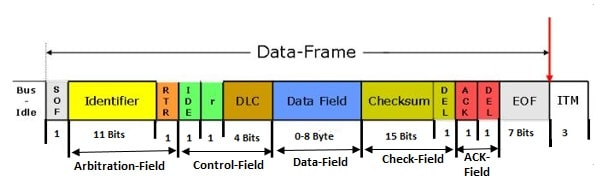
\includegraphics[width=\textwidth]{obrazky/can_frame}
    \caption{CAN bus frame with standard identifier~\cite{piembsystech_can_nodate}.}
    \label{fig:can_frame}
\end{figure}

An important bit for CANOpen is the RTR bit, which stands for Remote Transmission Request, when this bit is recessive, there are no data contained in the frame and the frame asks the remote device for data.
As can be seen in the figure, the identifier and the RTR field are part of an Arbitration field, these bytes are used in the shared medium collision detection and control and thanks to this field, frames with lower ID have higher priority in the transmission.

\subsection{I\textsuperscript{2}C}
\label{subsec:i2c}
I\textsuperscript{2}C (Inter-Integrated Circuit) bus is a bus, that allows connecting multiple peripheral (slave) ICs to a controller (master) IC (multi-master mode is also supported)\cite{sfuptownmaker_i2c_2021}.
Hardware-wise the bus utilizes two pins in open collector configuration, which means that the high-level voltage need to be provided externally using a Pull-Up resistor.
The resistance value of the Pull-Up resistor affects the bus performance and can be fine-tuned to compensate for the parasitic capacity for the wiring.
Open-Collector configuration also means that when idle, the bus is pulled up to the defined voltage level and when the device want to transmit data, they can only pull the signal down.
The I\textsuperscript{2}C bus consists of two signals - the data signal (SDA) and the clock signal (SDA).

The I\textsuperscript{2}C transaction begins when the controller sends START condition on the bus, the START condition is followed by the peripheral device address, and a direction bit determining whether the controller wants to write or read from the peripheral device\cite{sfuptownmaker_i2c_2021}.
Then based on the direction bit the controller either receives data or sends them.
The peripheral has a mechanism of stopping the clock signal in an event the peripheral is not fast enough to produce data, that is done by pulling the clock signal low and then releasing it when the data re available.
When the data is transferred, the controller finalizes the transfer by sending the STOP condition.

When interfacing with various peripherals, the read and write transactions are combined\cite{valdez_understanding_2015}.
The controller first sends the peripheral address (with direction bit set to write) followed by the register it wants to access, the register is ACKed and now the controller either sends the data to be written or issues a Repeated START, transmits peripheral address with direction bits set to read and awaits data from the peripheral.
Writing to a peripheral using this approach can be seen in the Figure~\ref{fig:i2c_w} and reading data can be seen in the Figure~\ref{fig:i2c_r}.

\begin{figure}[H]
    \centering
    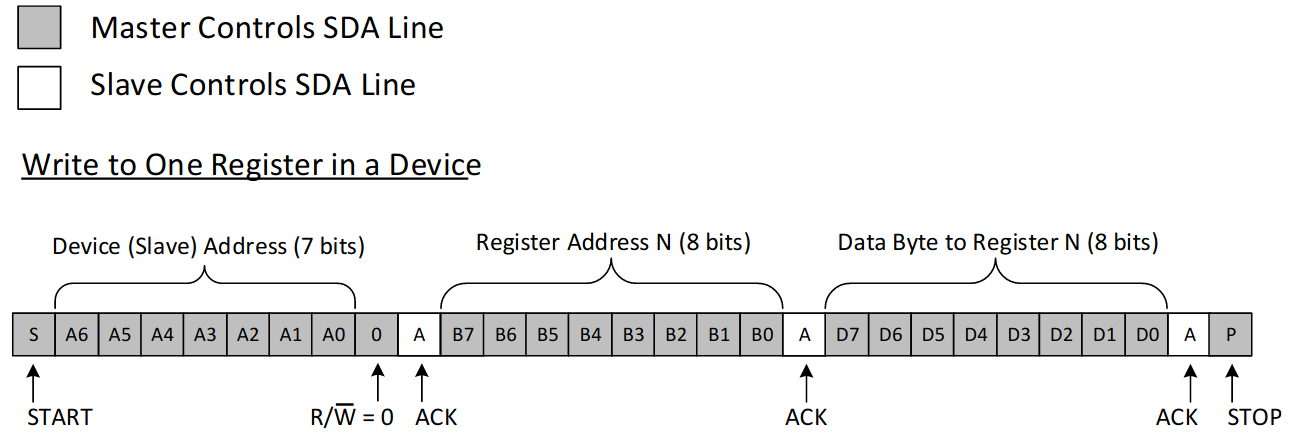
\includegraphics[width=\textwidth]{obrazky/i2c_w}
    \caption{Writing to a register of an I\textsuperscript{2}C peripheral IC~\cite{valdez_understanding_2015}.}
    \label{fig:i2c_w}
\end{figure}

\begin{figure}[H]
    \centering
    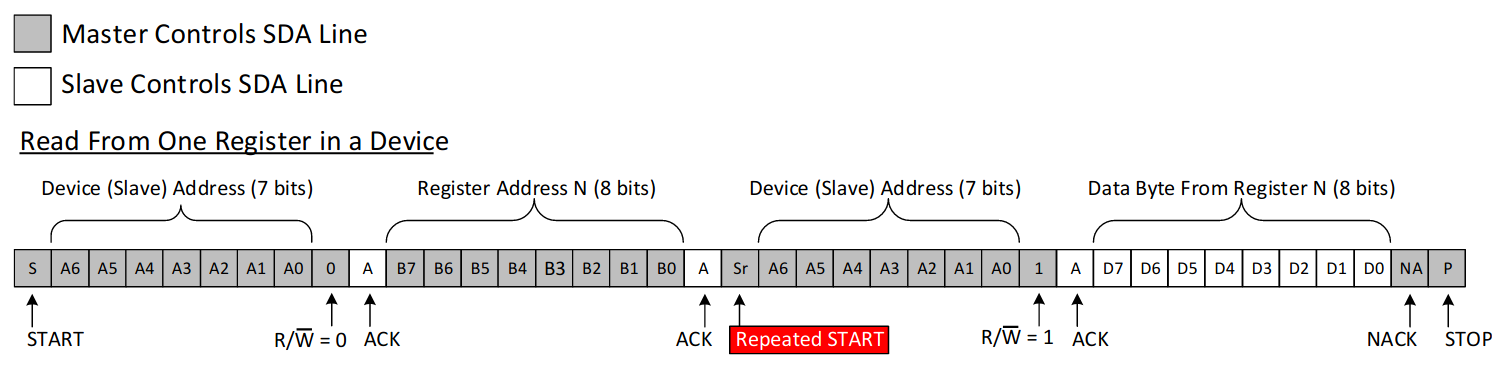
\includegraphics[width=1.1\textwidth]{obrazky/i2c_r}
    \caption{Reading a register of an I\textsuperscript{2}C peripheral IC~\cite{valdez_understanding_2015}.}
    \label{fig:i2c_r}
\end{figure}

\subsection{Universal Serial Bus}
\label{subsec:usb}
USB (Universal Serial Bus) utilizes a differential pair (or multiple) for data transfer.
Nowadays, USB devices are ubiquitous and perform variety of different functions and according to these functions are separated into classes (Mass Storage, HID (Human Interface Devices), etc.).
Through the time, there were four major revisions of the USB standard as can be seen in the Table~\ref{tab:usb}.

\begin{table}[H]
    \centering
    \begin{tabular}{ |c|c|c| }
        \hline
        Version & Max. Data Rate & Code Name \\
        \hline
        \hline
        1.0 & 1.5 Mbit/s & Low Speed \\
        \hline
         & 12 Mbit/s & Full Speed \\
        \hline
        2.0 & 480 Mbit/s & HighSpeed \\
        \hline
        3.0 & 5 Gbit/s & SuperSpeed \\
        \hline
        3.1 gen 2 & 10 Gbit/s & SuperSpeed+ \\
        \hline
        3.2 & 20 Gbit/s & SuperSpeed+ USB dual-line \\
        \hline
        4.0 & 40 Gbit/s &  \\
        \hline
    \end{tabular}
    \caption{USB versions and data rates~\cite{noauthor_usb_2021}}
    \label{tab:usb}
\end{table}

USB is nowadays everywhere, with different supported transfer data rates, different utilization of connectors etc.
With such diverse use cases and device, the whole USB ecosystem is increasingly more difficult to orient within.
For our use case, we'll be utilizing the USB controller present on the MCU, which is a USB 2.0 OTG (On The Go) Full Speed device\cite{stmicro_an4879_2018}, but in order to support better compatibility and mechanical properties, we'll be using the USB-C receptacle with both lanes interconnected.